\documentclass[12pt,a4paper]{article}
\usepackage{indentfirst}
\usepackage{fontspec}
\usepackage{graphicx}
\usepackage{float}
\usepackage{subfigure}
\usepackage{wrapfig}
\setmainfont{Times New Roman}
\begin{document}
\begin{titlepage}
   \begin{center}
       \vspace*{1cm}

       \textbf{\Huge{Music Feature}}

       \vspace{0.5cm}
        \Large{Music Genre Classification}
            
       \vspace{1.5cm}

       \textbf{Yi-Hsin Lu}

       \vfill
            
        Statistical Machine Learning Final Presentation
            
       \vspace{0.8cm}
     
       \includegraphics[width=0.4\textwidth]{NDHU_logo.png}
            
       National Dong Hwa University\\
       2022 June 19
   \end{center}
\end{titlepage}

\tableofcontents

\newpage

\section*{Abstract}
Music genre can be predict by using Fourier transform and waveform analysis from audio to numerical data. For the model I used like SVM and Random Forest, the result was better than the others in Kaggle.


\section{Introduction}
\subsection{Motivating Question}
When I was a child, I started learning chinese music instrument. That was the beginning that having fun for the music, and I realized the music is also a part of science. For an example, A440 is the musical pitch corresponding to an audio frequency of 440 Hz(from Wikipedia), and every instruments have their own waveform. So I decided to have my master degree that I want to use my statistics knowledge on the music I learned before. The music topic is the work direction for statistical machine learning project.

\subsection{Focus Problem}
A dataset in Kaggle interests me, 1000 audio tracks each 30 seconds long, it contains 10 genres, each represented by 100 tracks. So my problem is:\\
1. Is the music genre classified by those numerical data?\\
2. If it can be classified, which model is the best  

\subsection{Data}
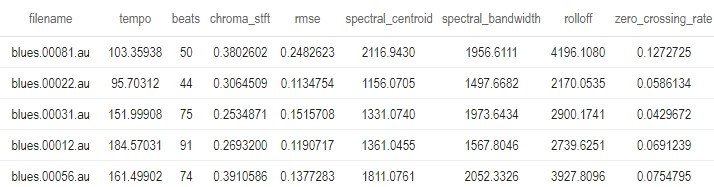
\includegraphics[width=0.8\textwidth]{data_head.jpg}\\
\\
The features in this dataset are extracted from the dataset provided it which consists of 1000 audio tracks each 30 seconds long. It contains 10 genres, each represented by 100 tracks. The tracks are all 22050Hz Mono 16-bit audio files in .wav format. The code used to extract features is at this GitHub repo. Features are extracted using libROSA library.(Content on kaggle)

\subsection{Variables/Features}
\begin{itemize}
  \item tempo: The speed at which a passage of music is played
  \item beats: Rhythmic unit in music
  \item chroma-stft: Short Time Fourier Transform
  \item rmse: Root Mean Square Error
  \item spectral-centroid: Indicates where the “center of mass” of the spectrum is located.
  \item spectral-bandwidth: It is the Wavelength interval in which a radiated spectral quantity is not less than half its maximum value.
  \item rolloff: Roll-off is the steepness of a transmission function with frequency.
  \item zero-crossing-rate: The rate at which the signal changes from positive to negative or back.
  \item mfcc1-20: Mel-frequency cepstral coefficients (MFCCs) are coefficients that collectively make up an MFC.
\end{itemize}

\subsection{Genre(label)}
\begin{itemize}
  \item blues
  \item classical
  \item country
  \item disco
  \item hiphop
  \item jazz
  \item metal
  \item pop
  \item reggae
  \item rock 
\end{itemize}

\newpage
\section{EDA}
\subsection{Correlation Matrix}
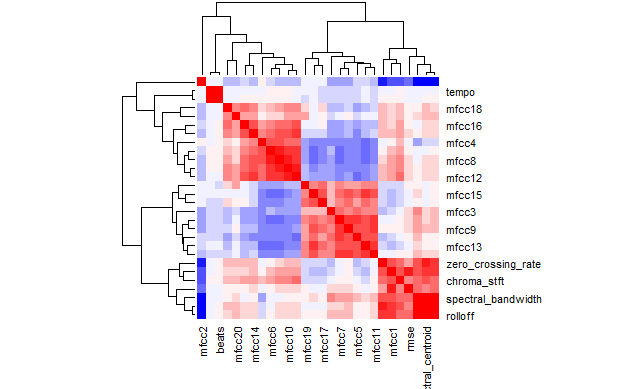
\includegraphics[width=1.2\textwidth]{correlation_matrix.png}
\\
It could be split by three parts in the red area that is the positive high correlation. Then we made the figure of pairs plot fir these three high correlation area.

\subsection{Pairs plot}
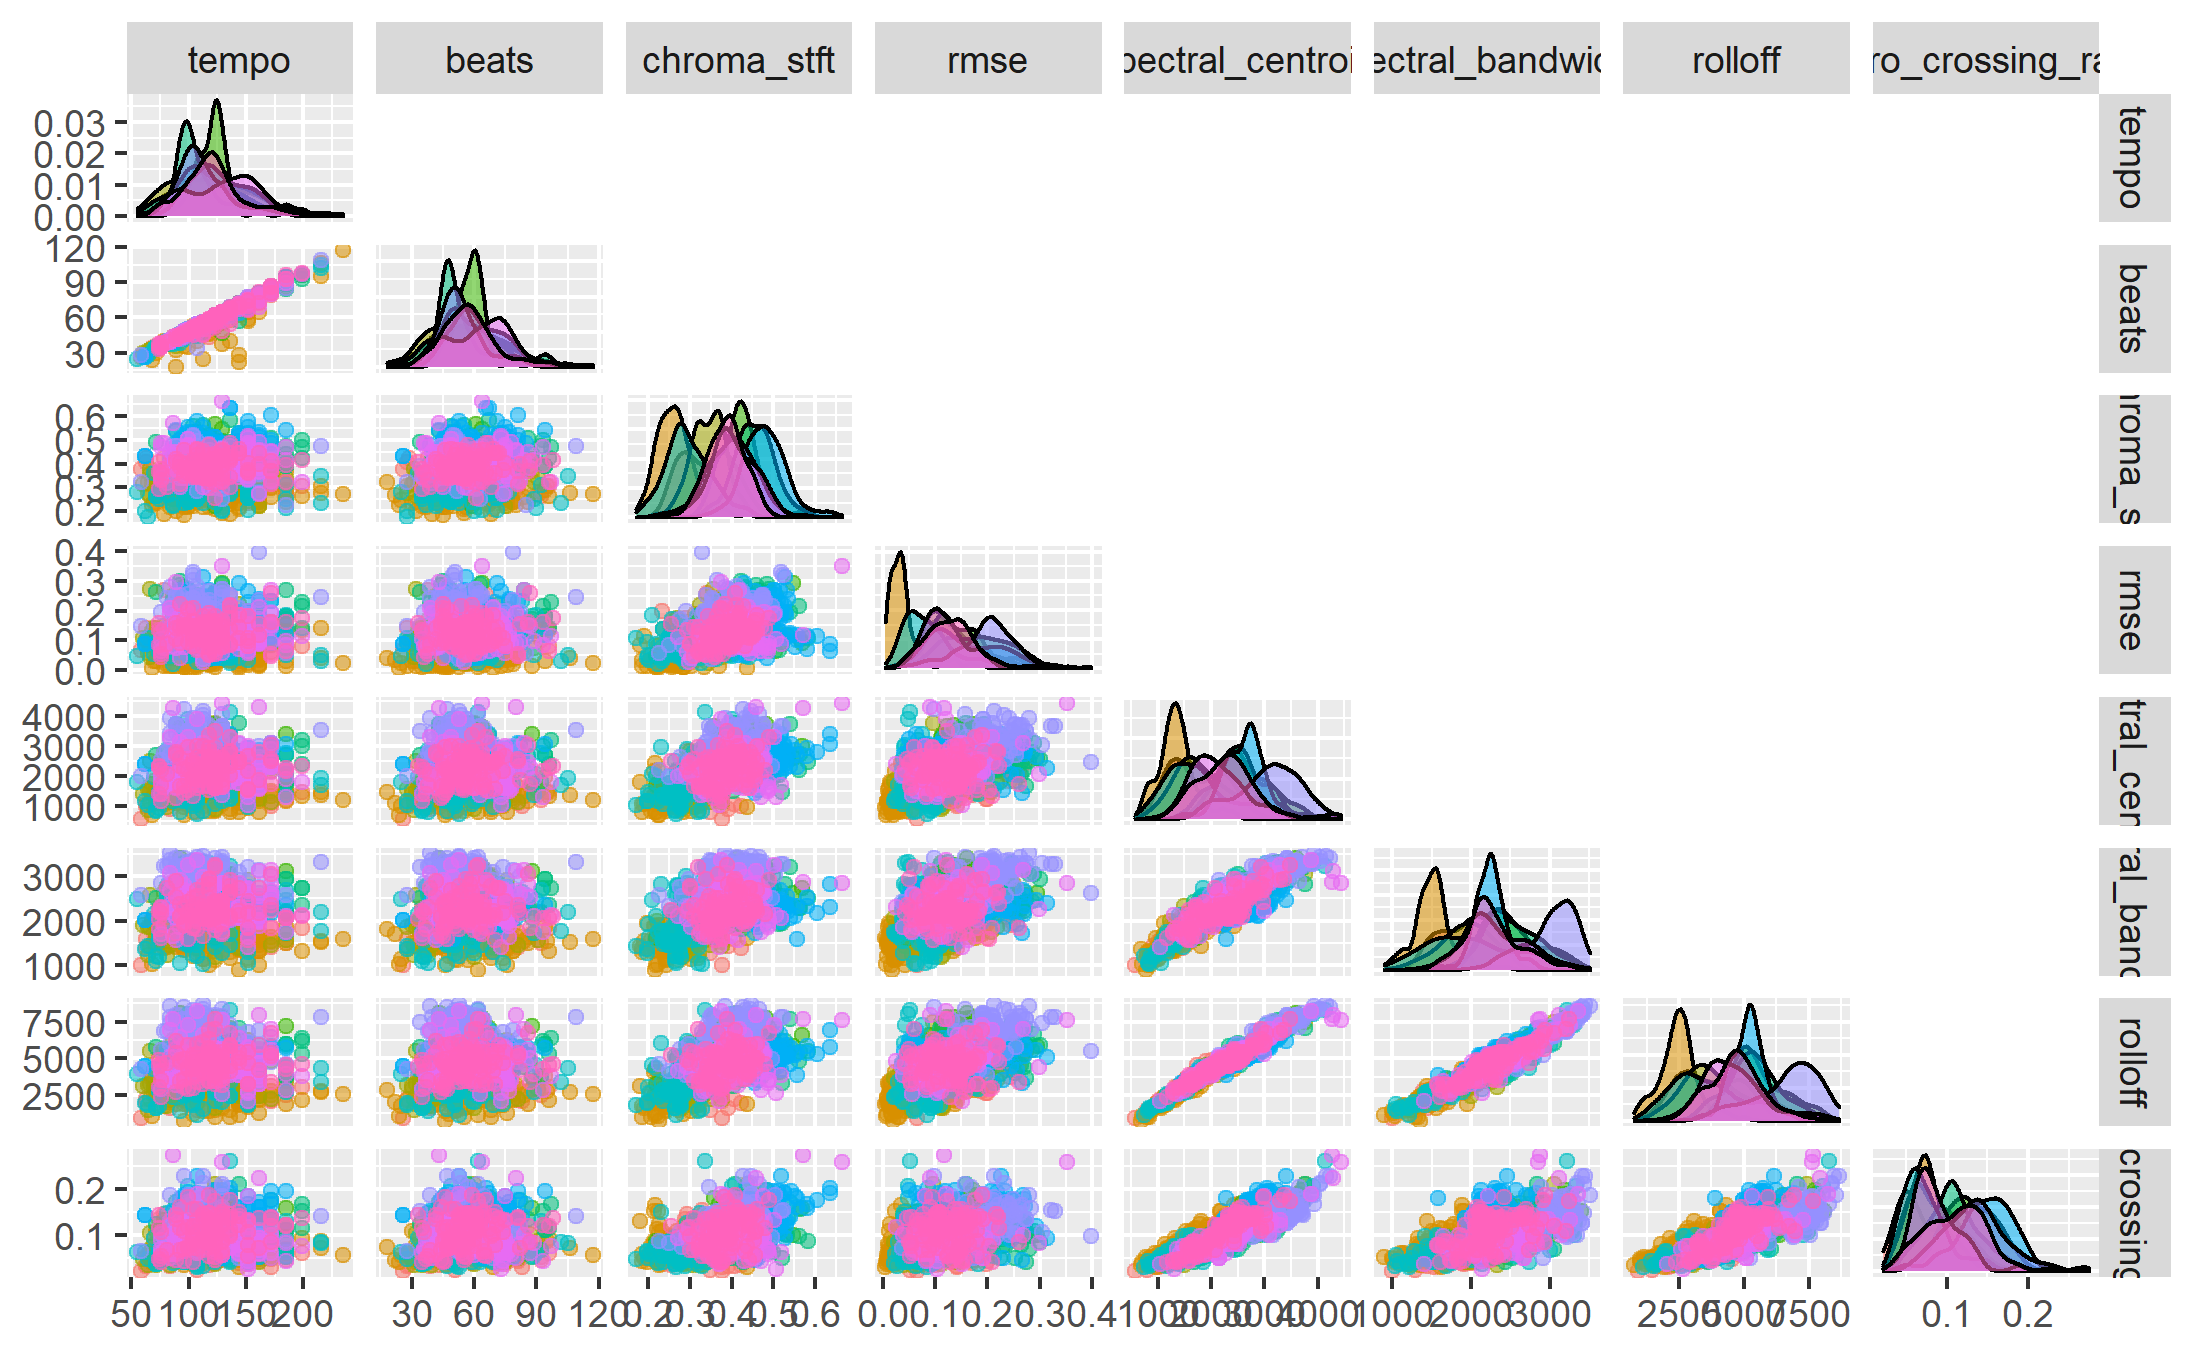
\includegraphics[width=0.35\textwidth]{ggpairs1.png}
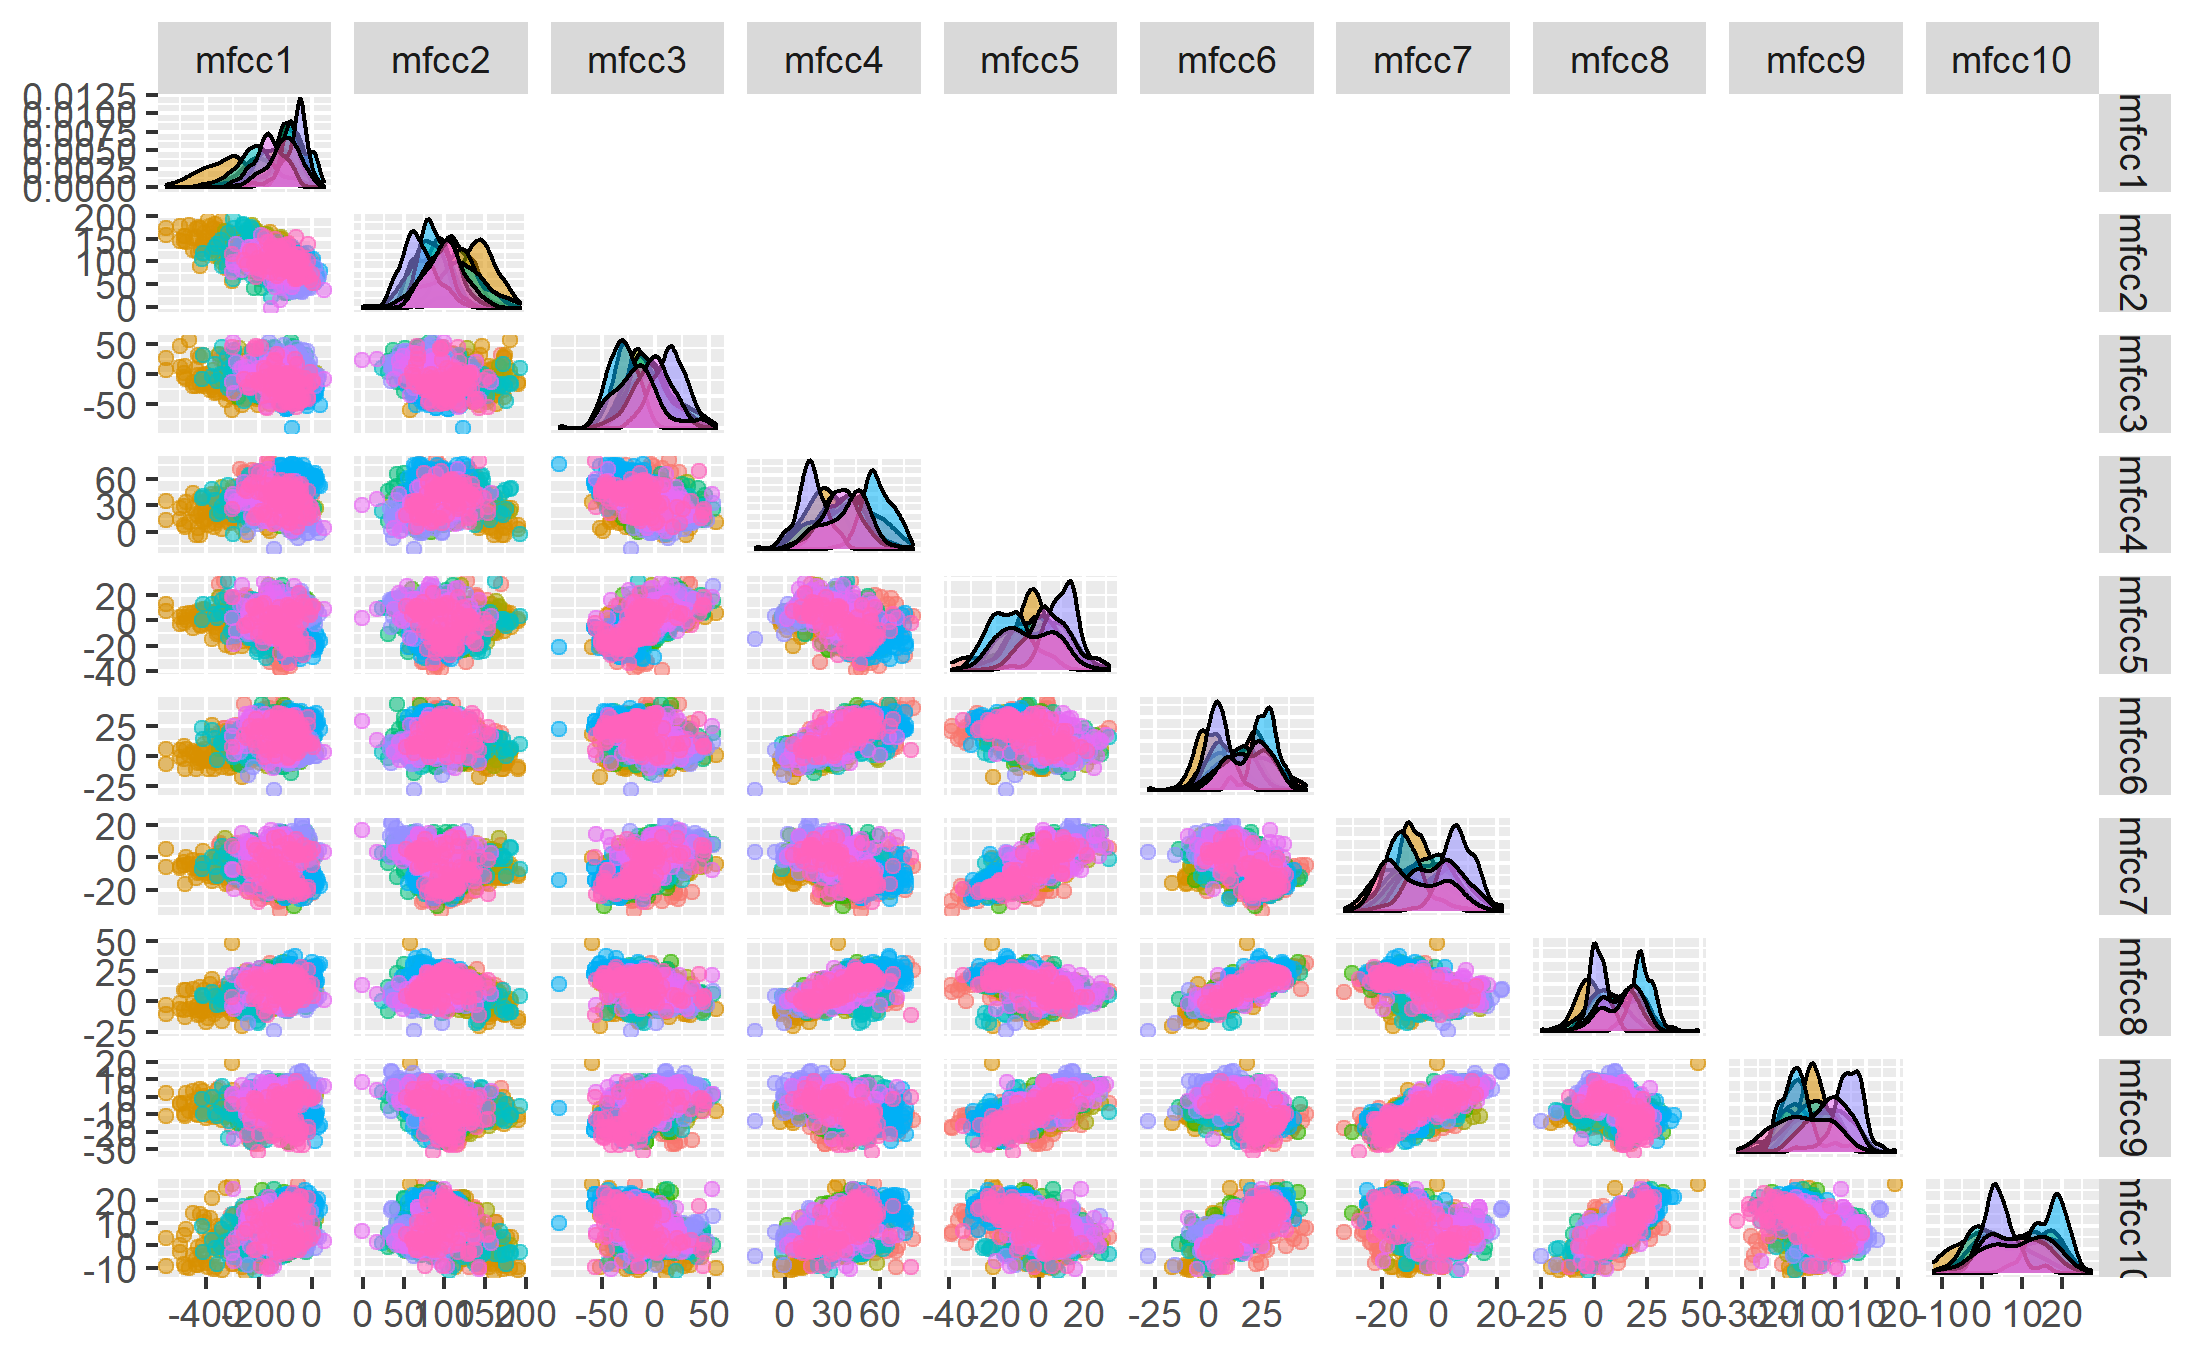
\includegraphics[width=0.35\textwidth]{ggpairs2.png}
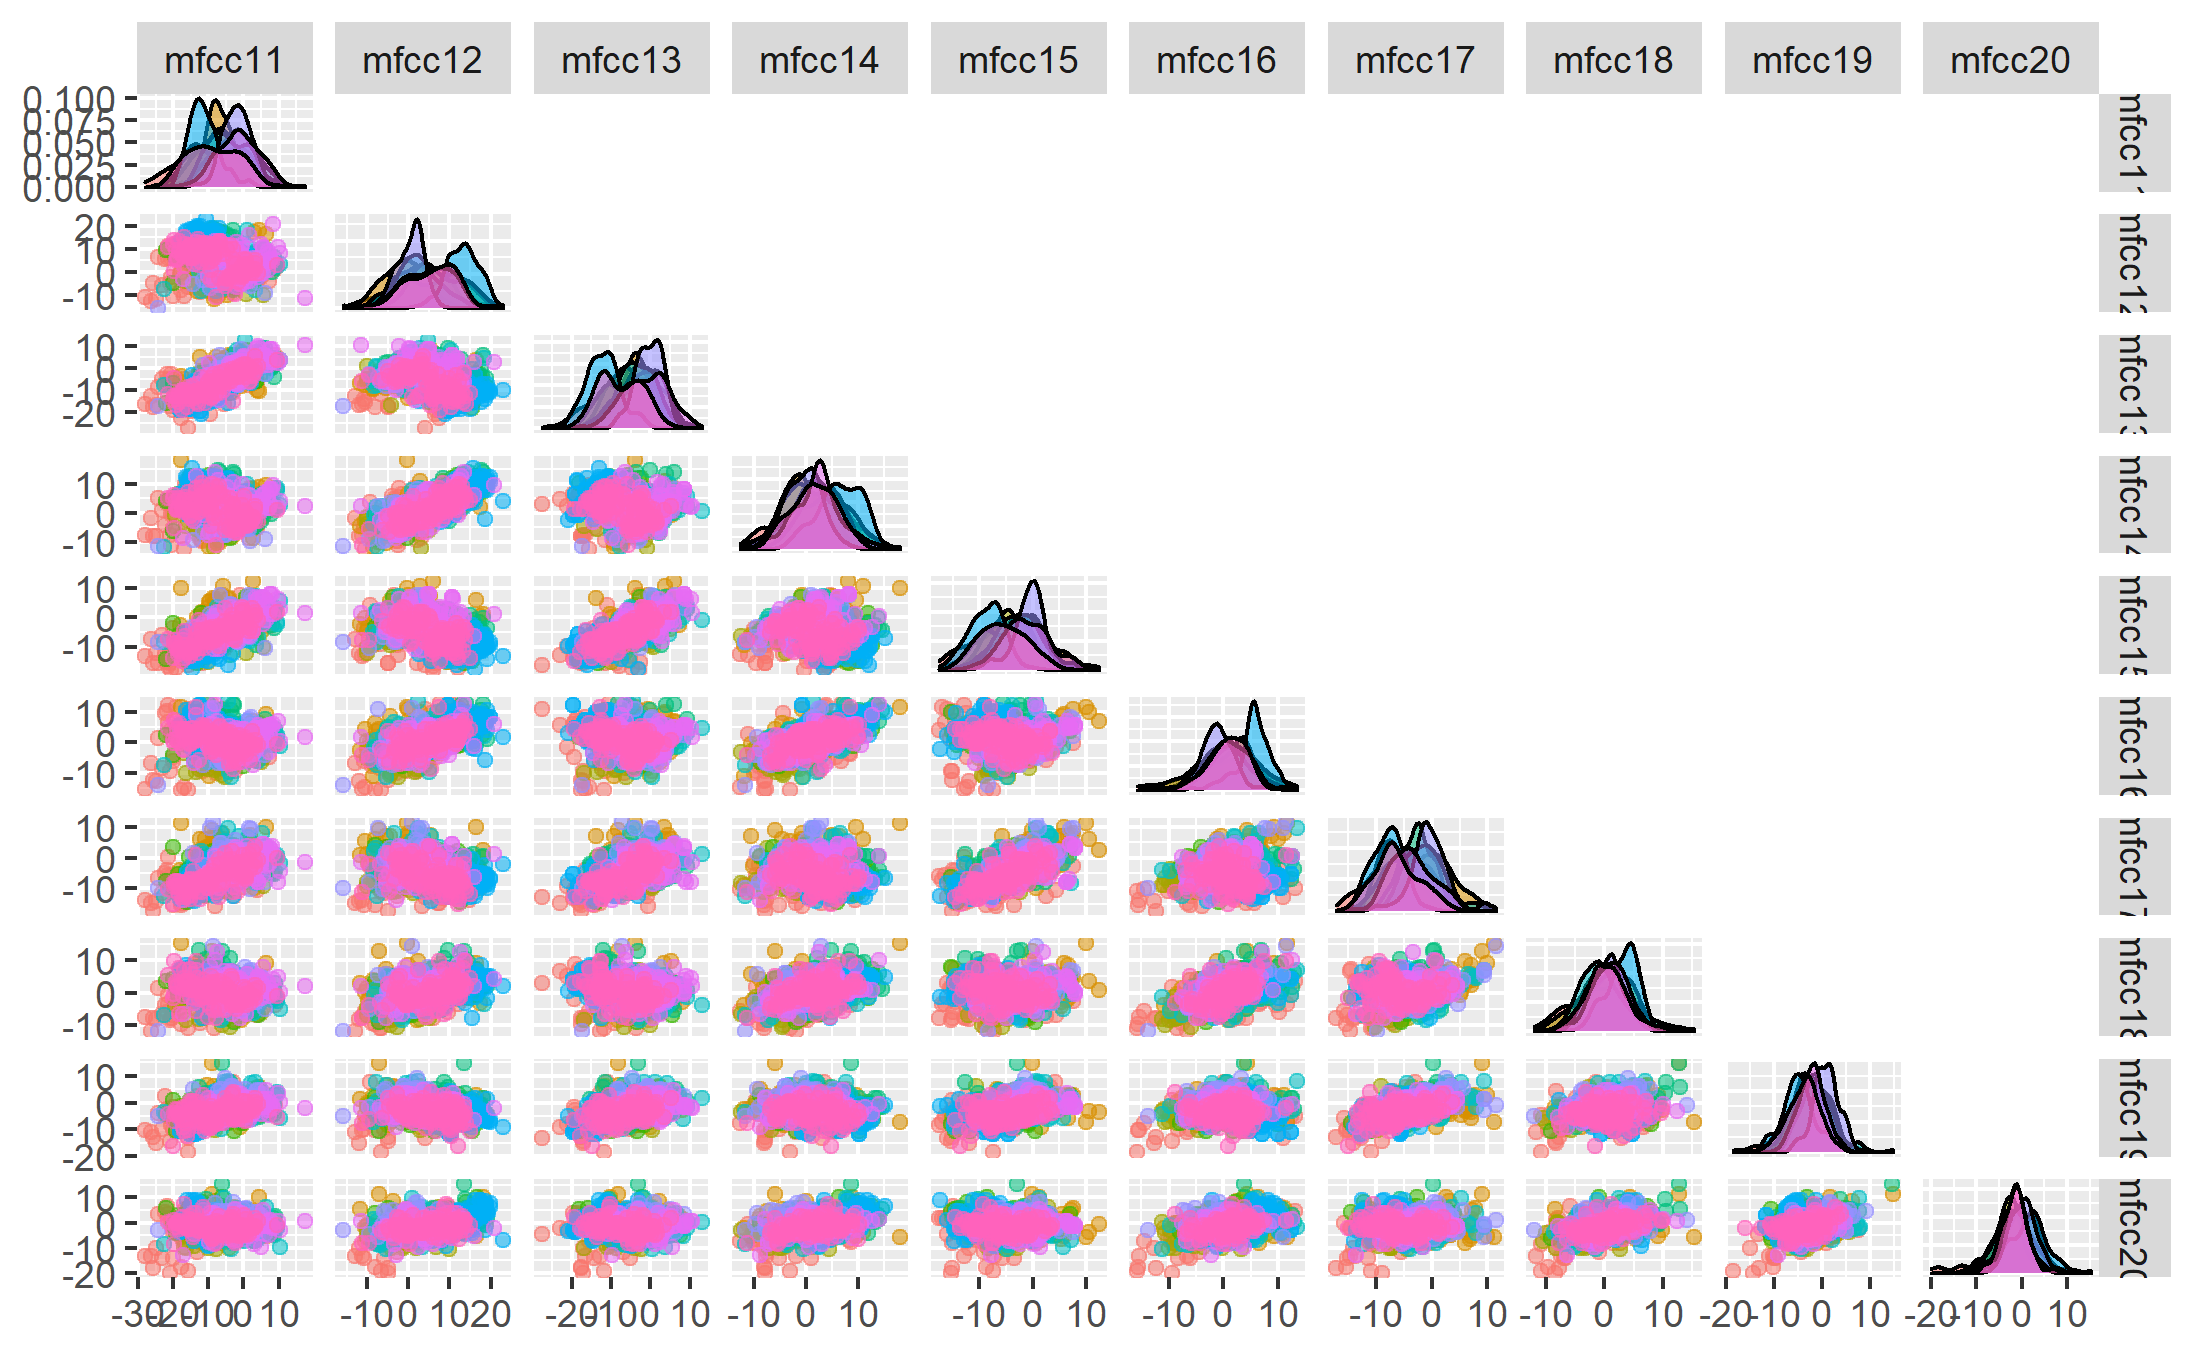
\includegraphics[width=0.35\textwidth]{ggpairs3.png}
\\
There is a high correlation between tempo and beats about 2 times. And spectral-centroid, spectral-bandwidth and rolloff are the results of spectral analysis, they must have correlation for each variables.

\newpage
\subsection{PCA(Principle Component Analysis)}
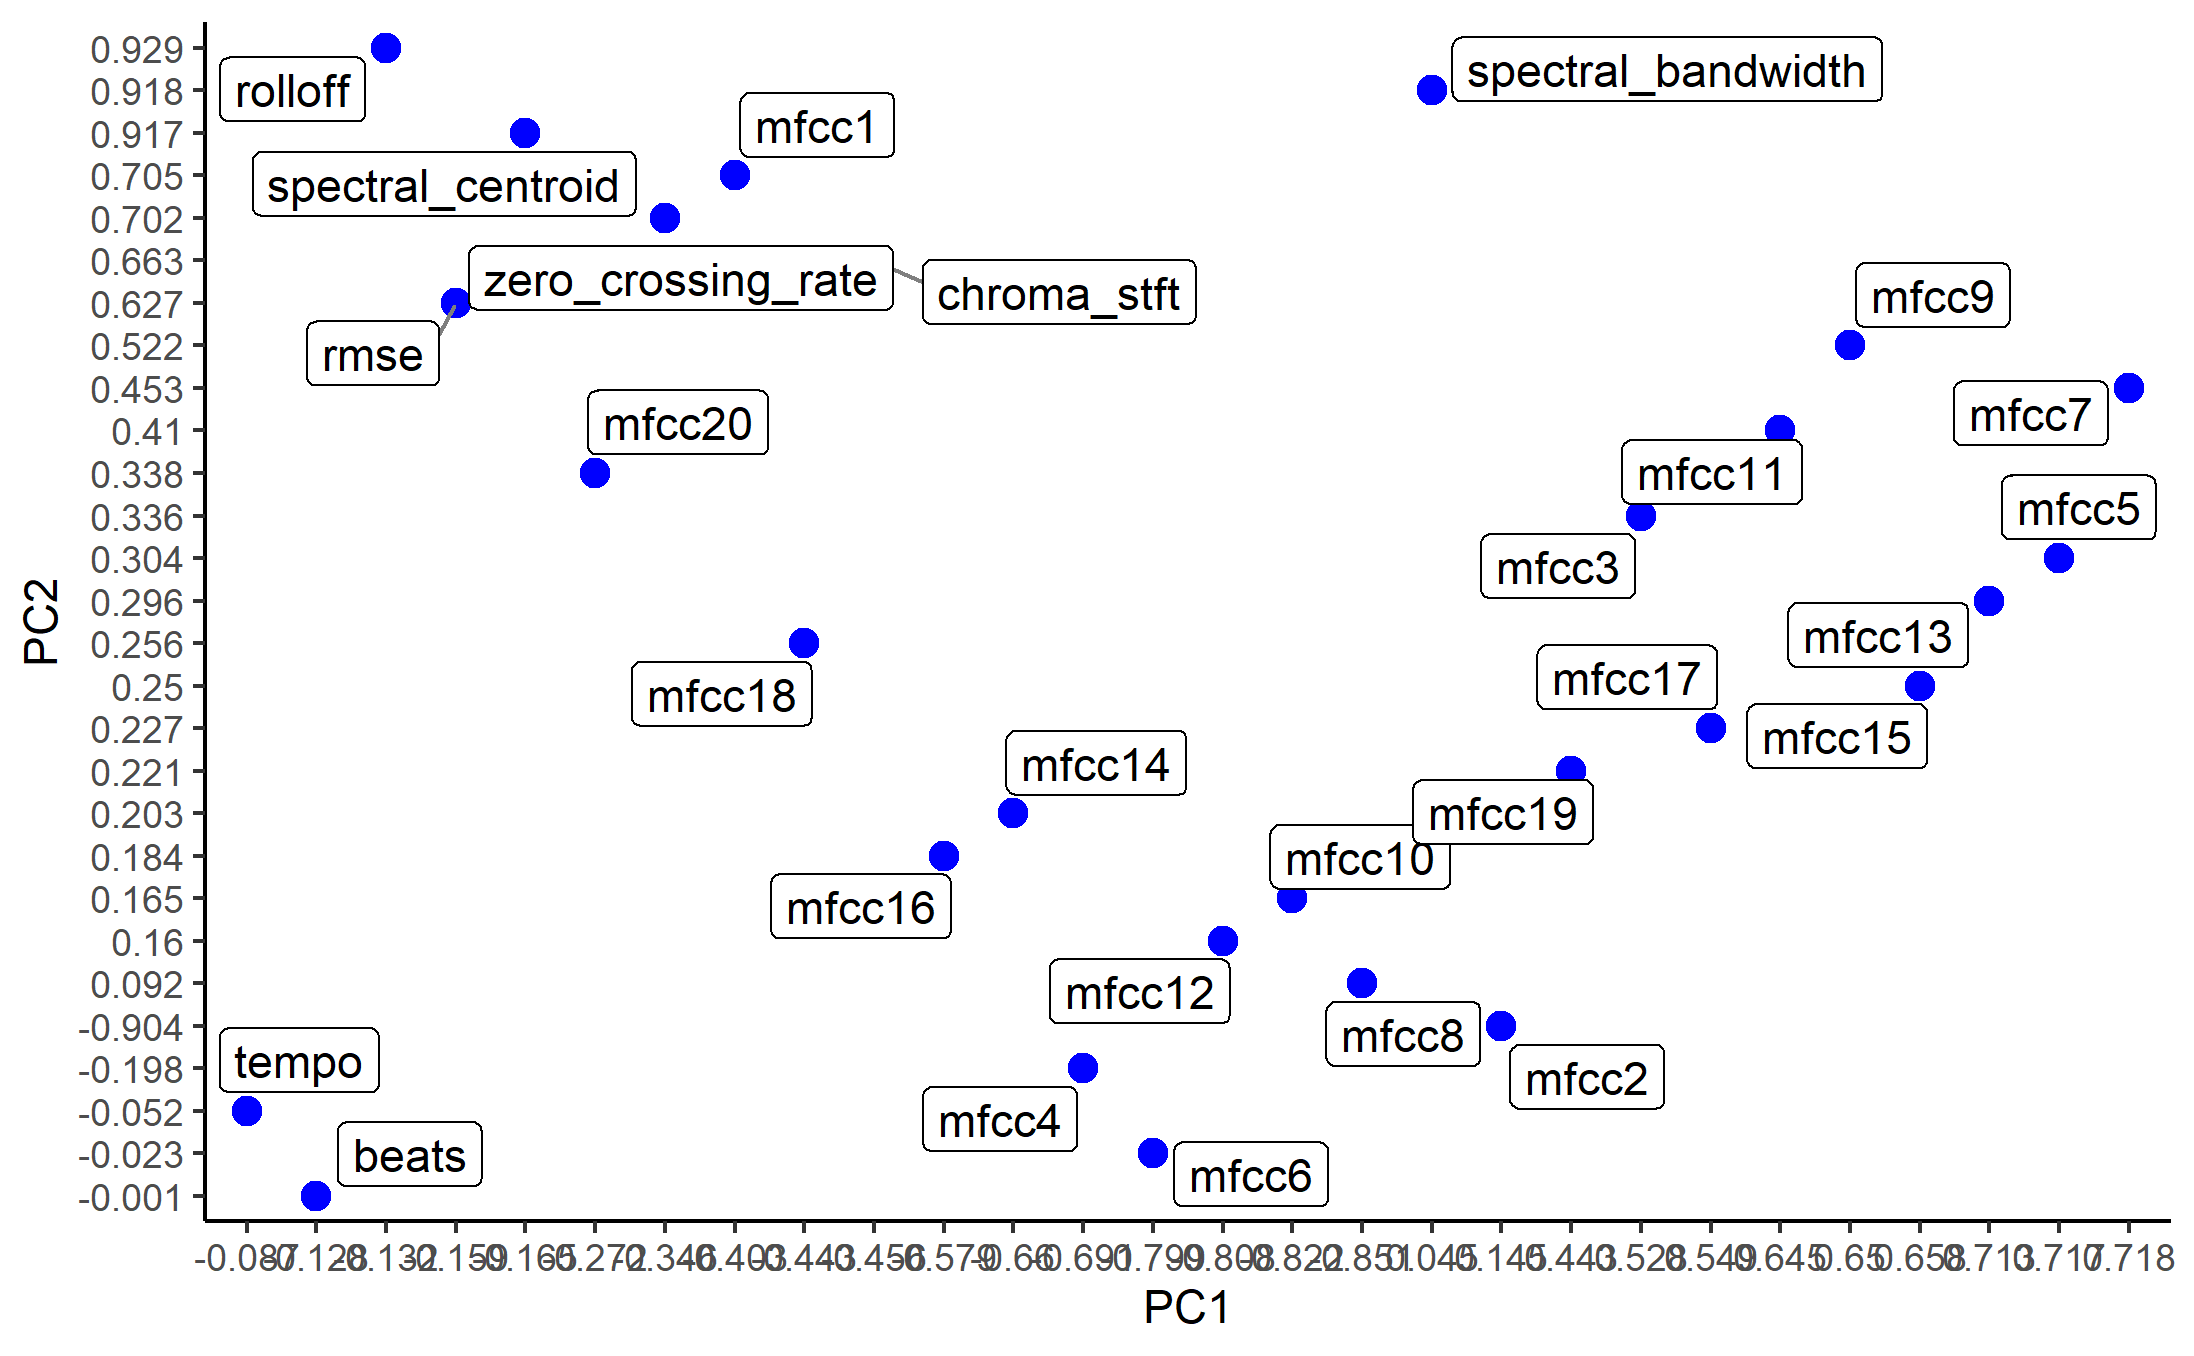
\includegraphics[width=0.5\textwidth]{pca_feat.png}
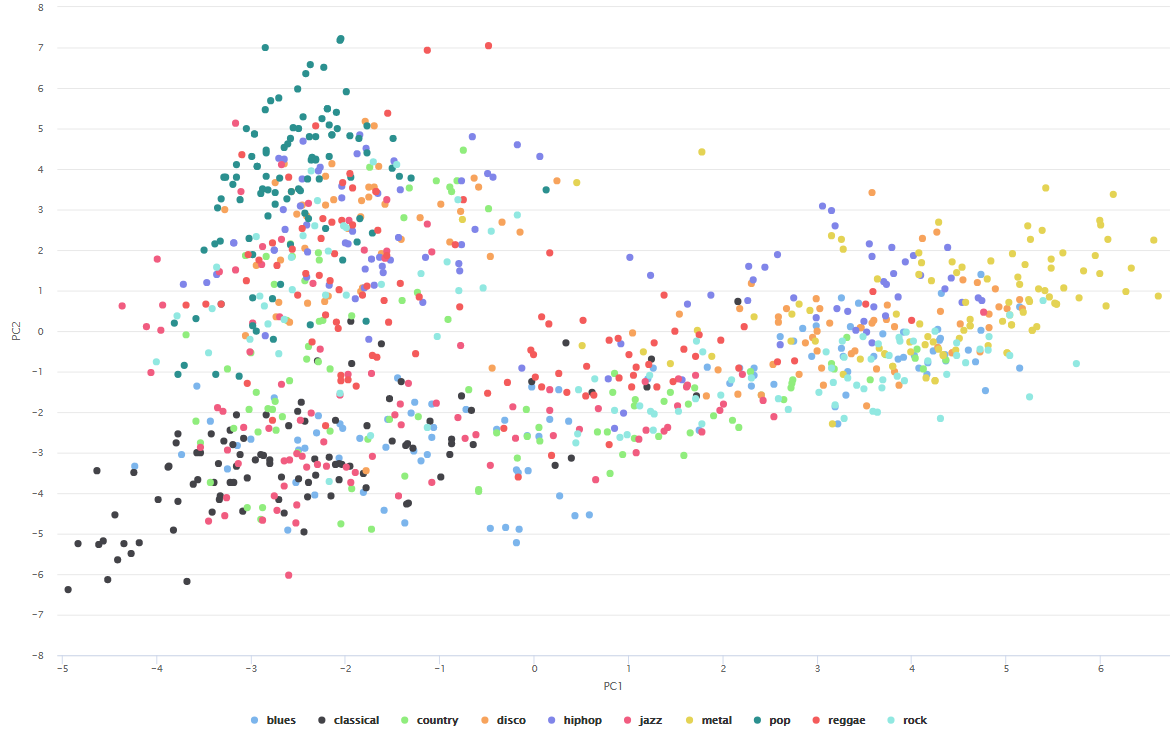
\includegraphics[width=0.5\textwidth]{pca.png}

\section{Models}
\subsection{Training and Testing data}
For the balance in this data, taking 80\% as training data and 20 \% as testing data from each genres, so training data contains 10 genres, each represented by 80 tracks. And so does testing data.

\subsection{Logistic Regression}
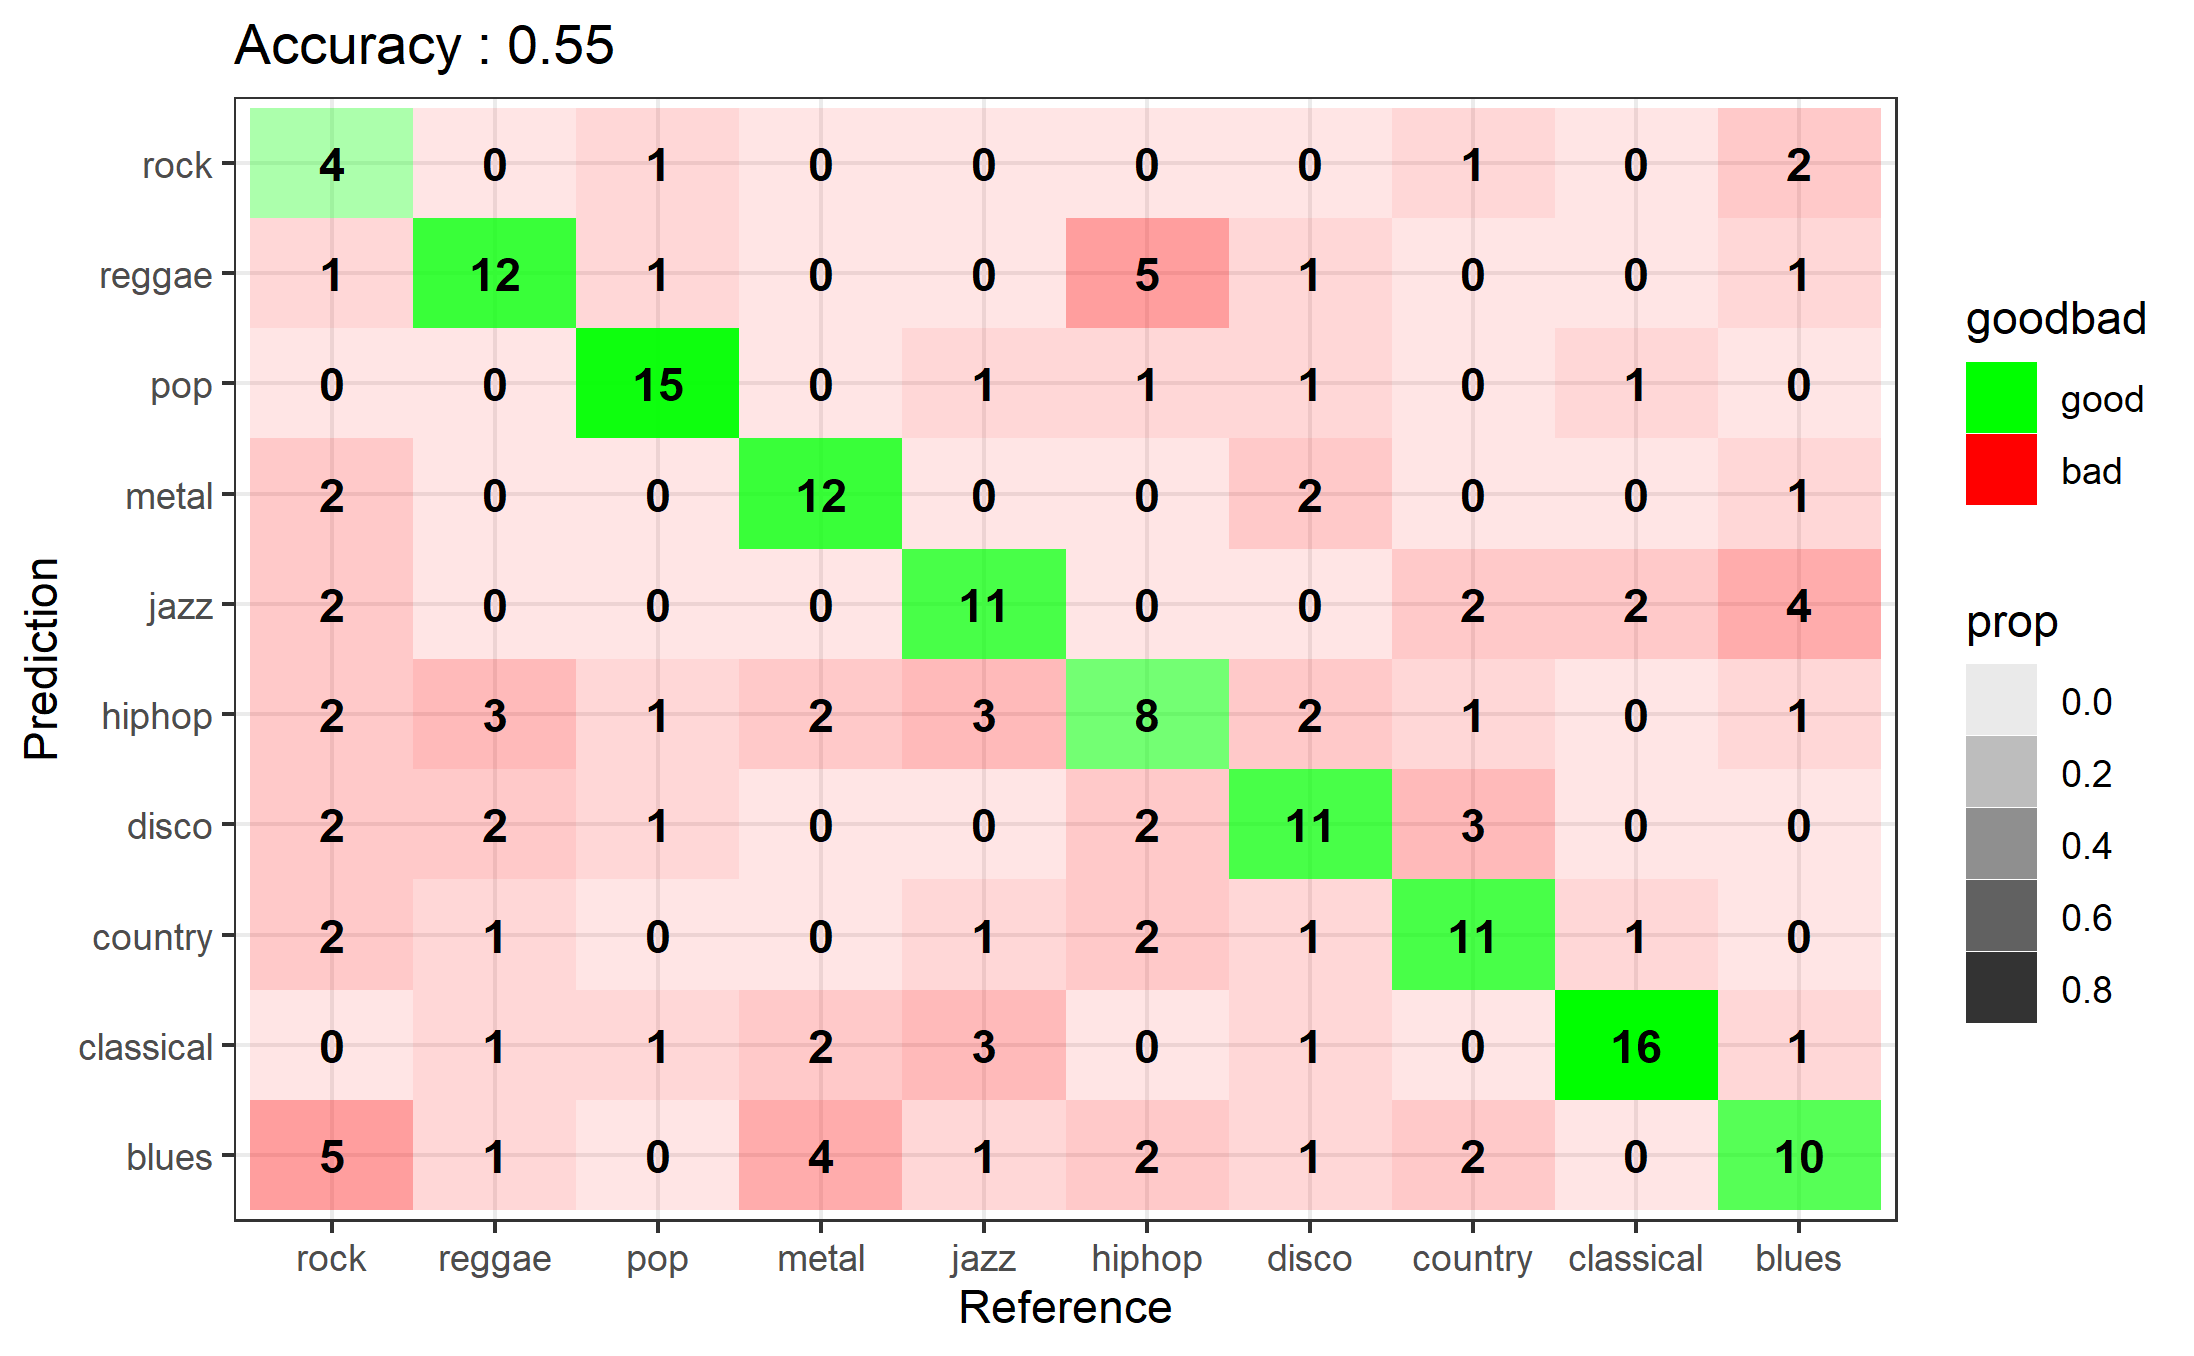
\includegraphics[width=0.9\textwidth]{confusionMatrix_logreg.png}
\newpage
\subsection{SVM(Support Vector Machine)}
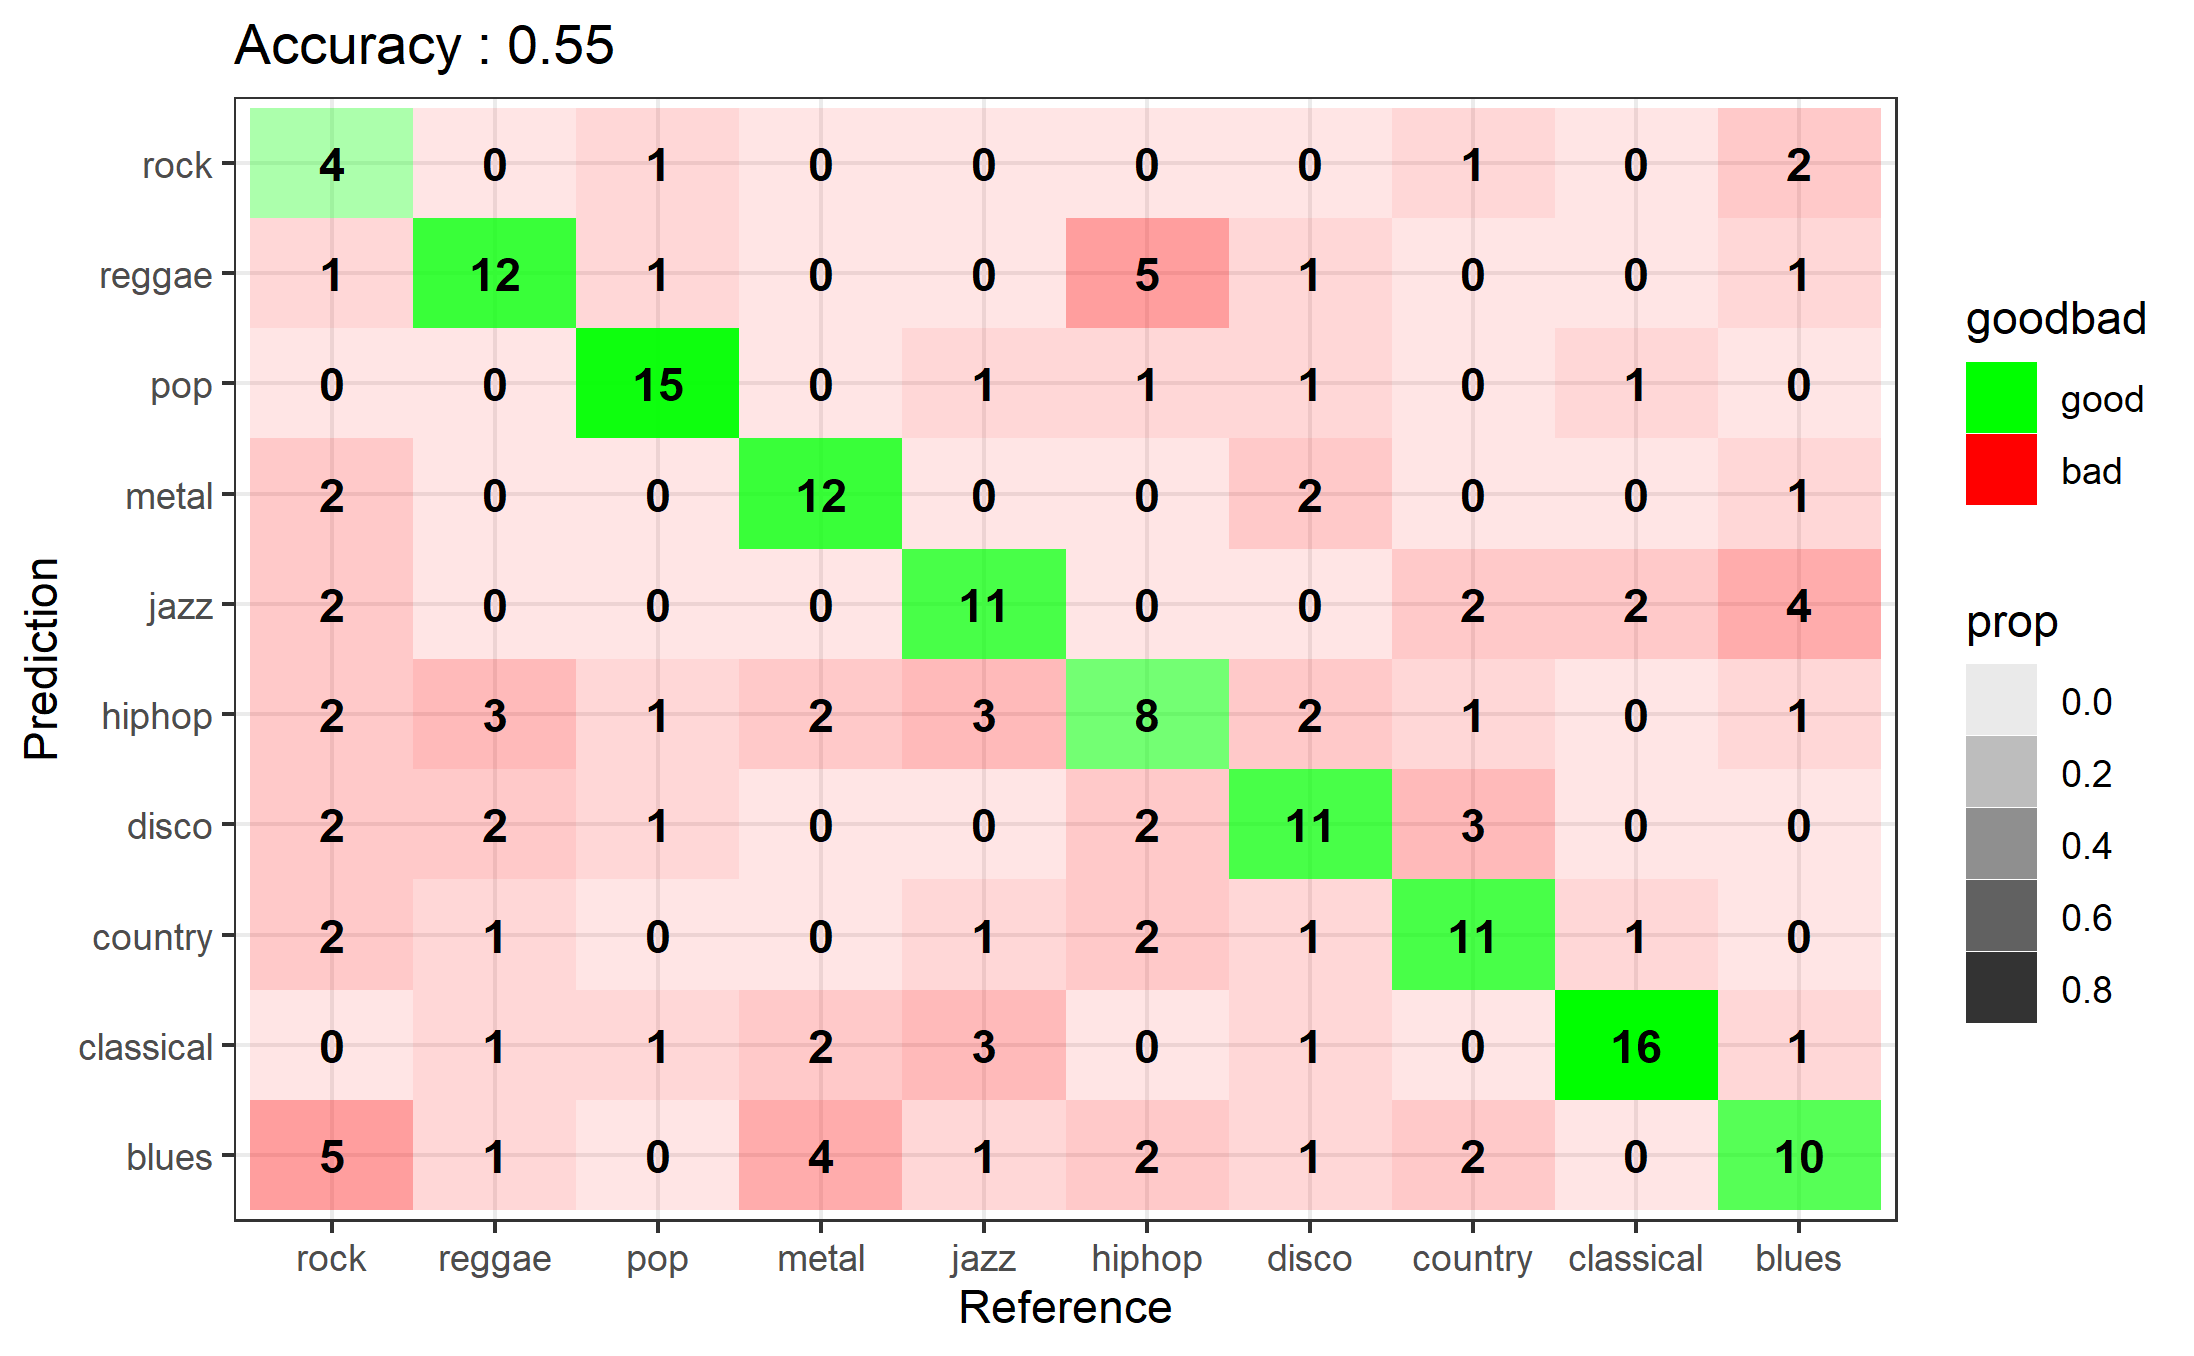
\includegraphics[width=0.9\textwidth]{confusionMatrix_logreg.png}
\subsection{SVM(one-hot encoding)}
Turning this 10 class prediction into a simple version, We do the one-hot encoding for the genres as the figure down below.\\
\begin{center}
    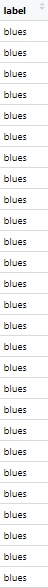
\includegraphics[width=0.05\textwidth]{y.jpg}$\Longrightarrow$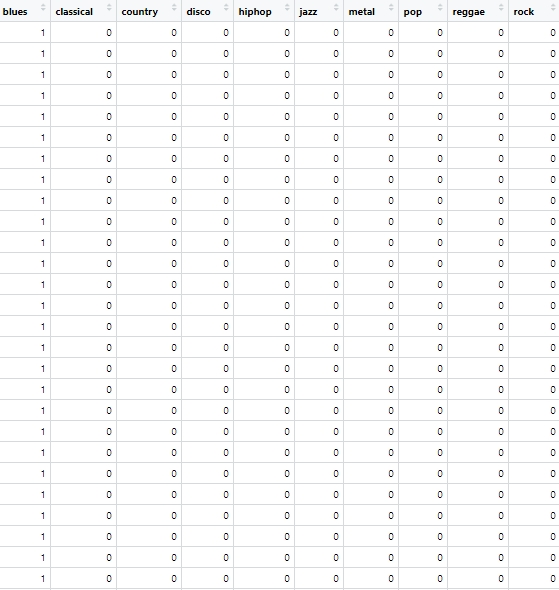
\includegraphics[width=0.6\textwidth]{y_matrix.jpg}
\end{center}
\newpage
Predict for each genres, and take the highest accuracy to be the predictor.\\
\\
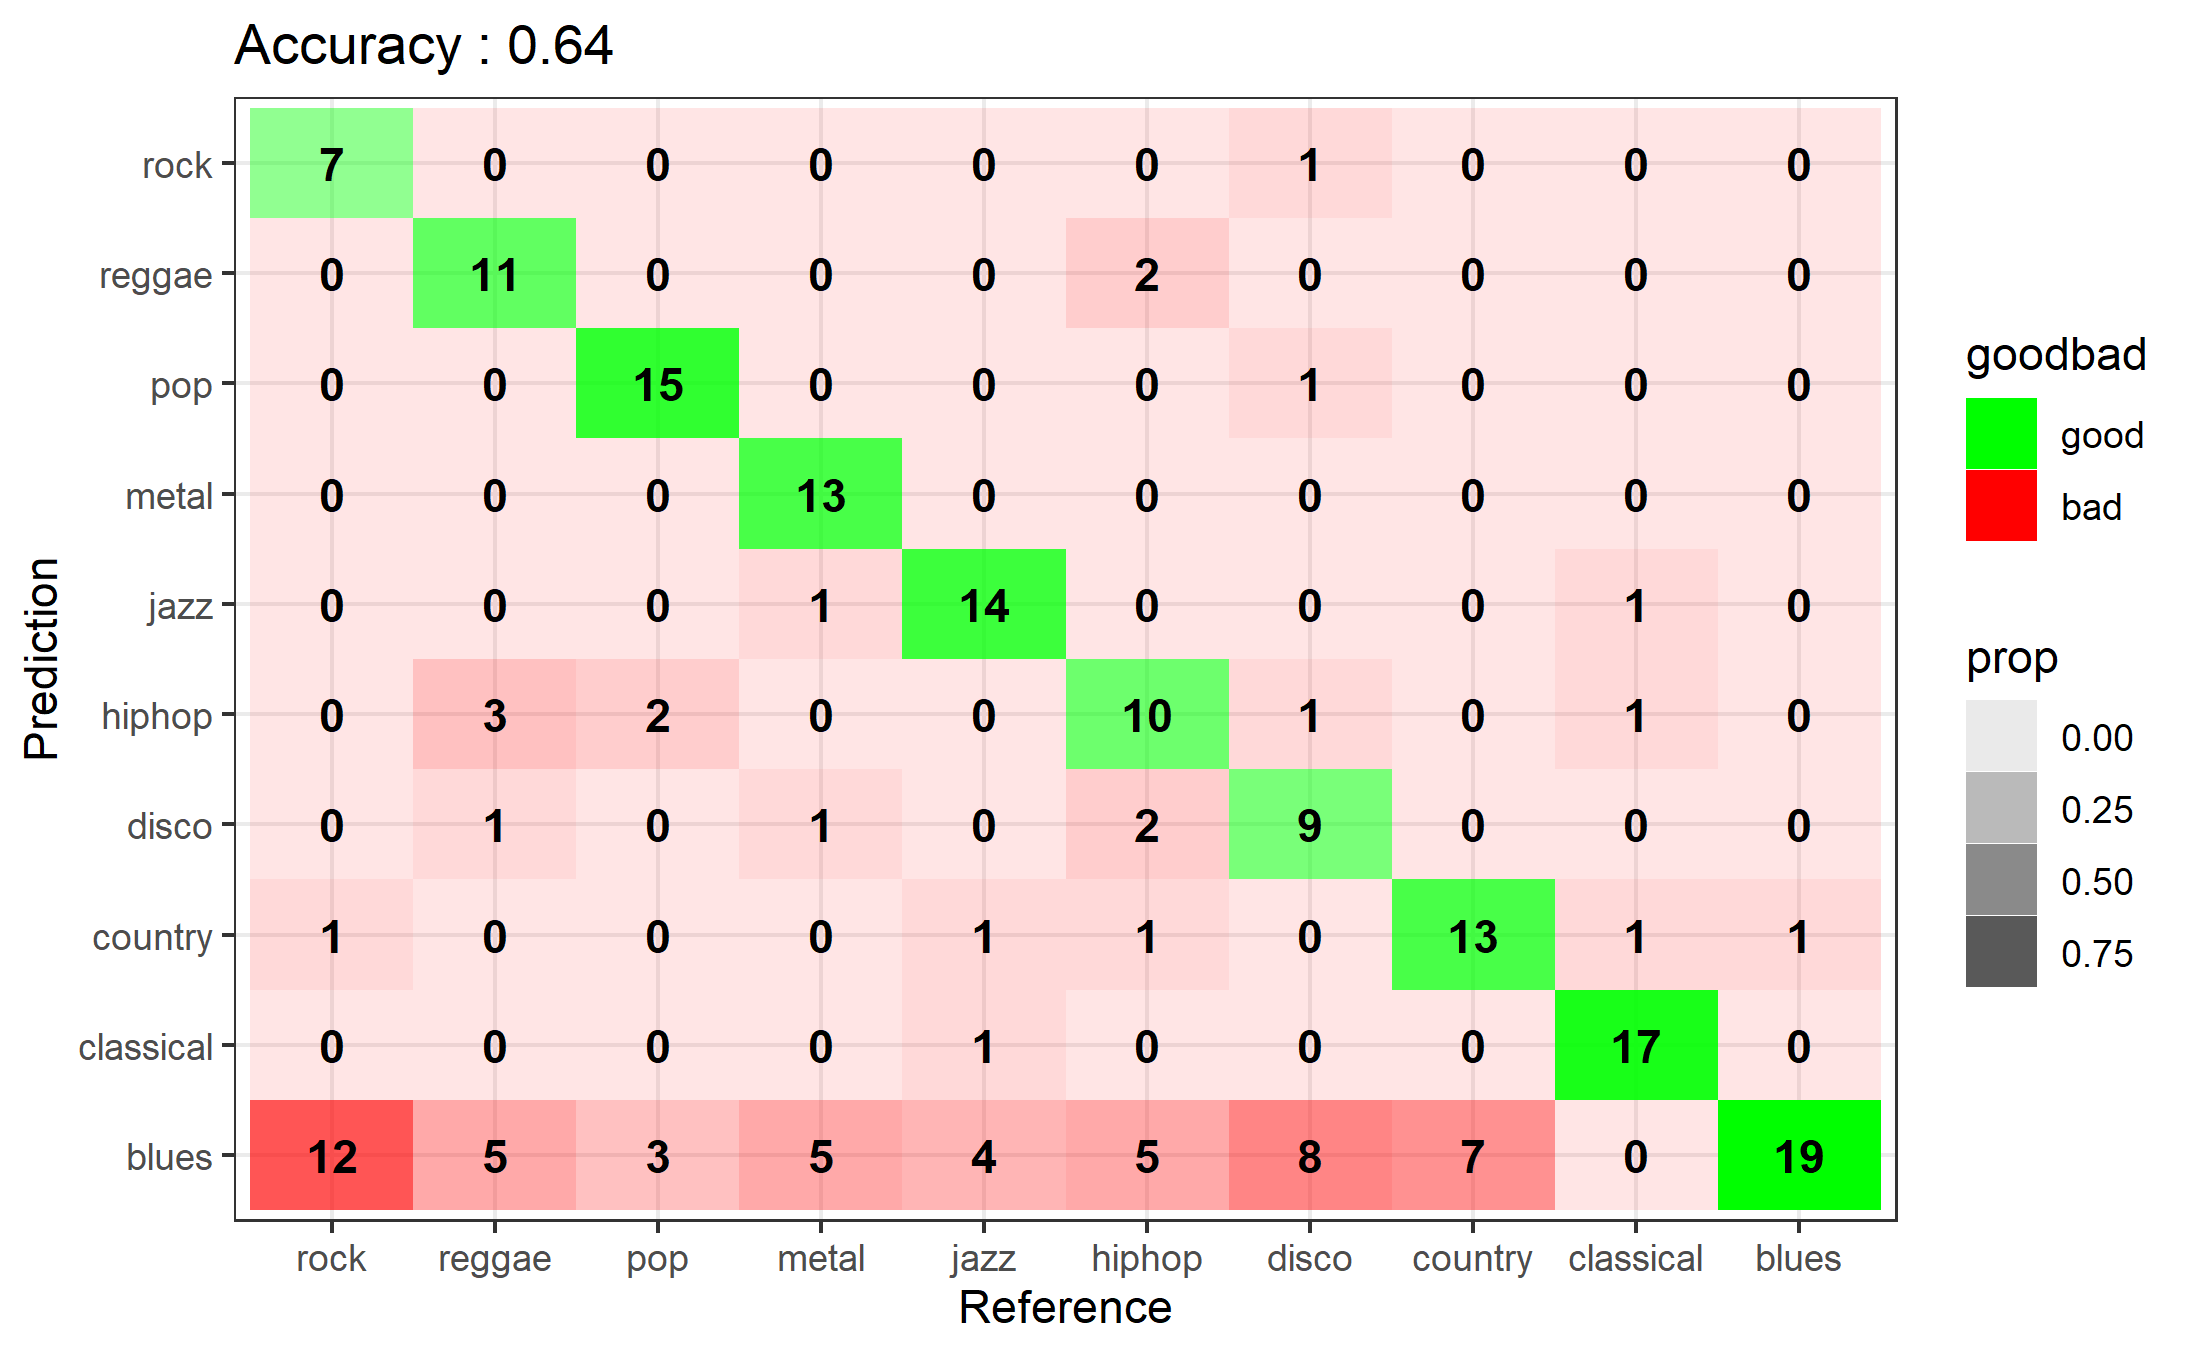
\includegraphics[width=0.9\textwidth]{confusionMatrix_ohencoding_std.png}
\subsection{SVM(scaling)}
After reading the paper of tuning of SVM, scaling is very essential.\\
\\
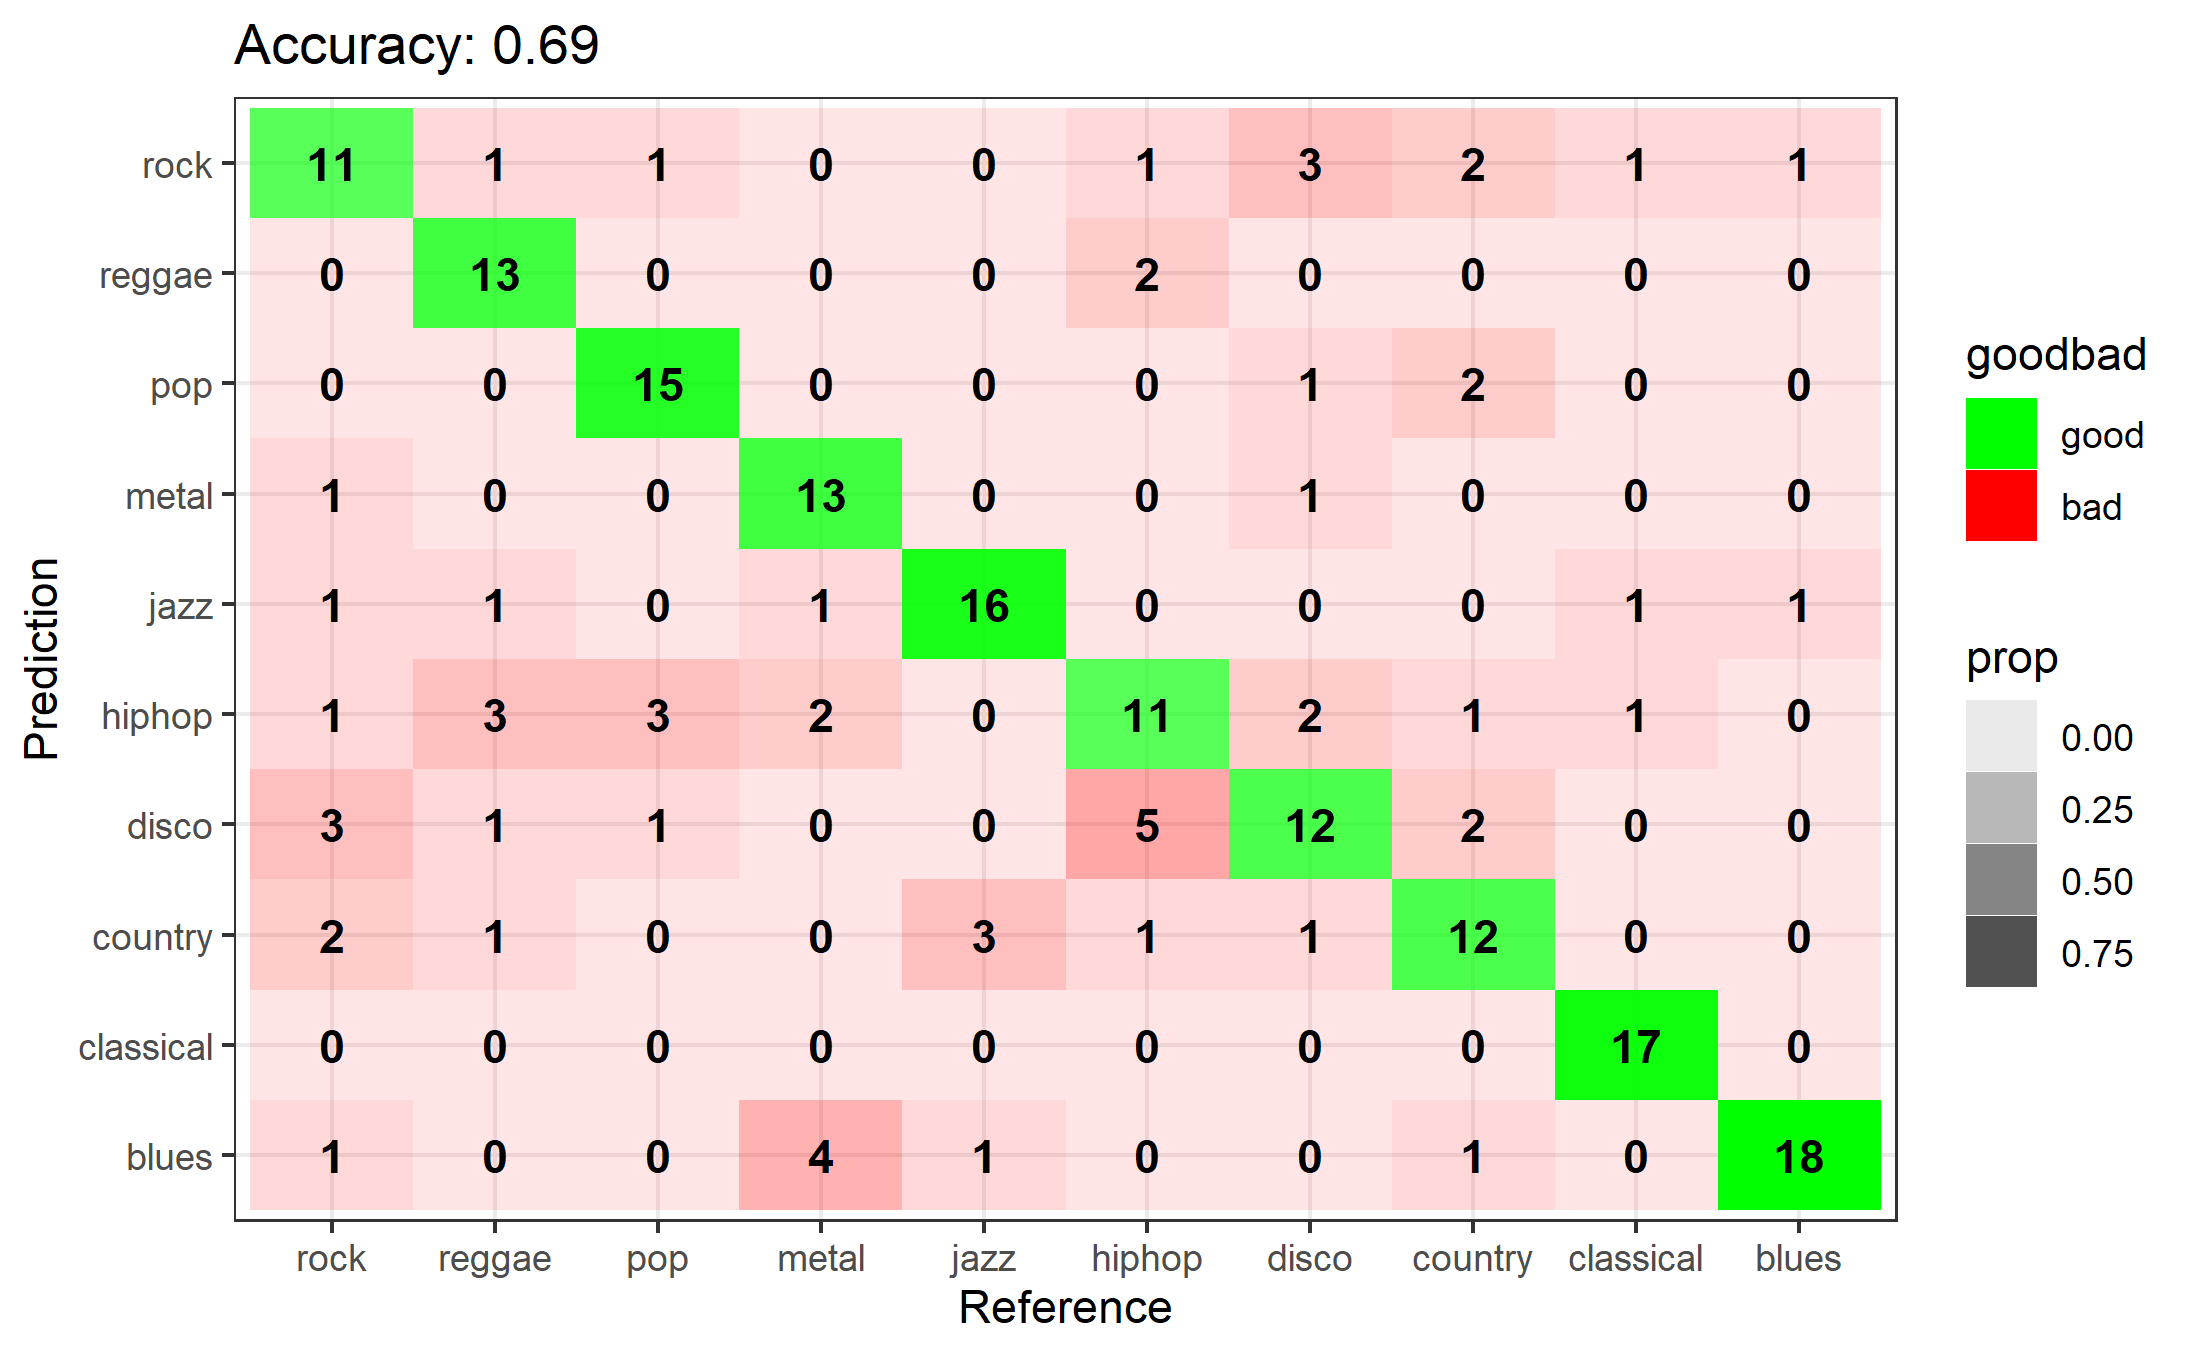
\includegraphics[width=0.9\textwidth]{confusionMatrix_svm_std.png}
\newpage

\subsection{Random Forest}
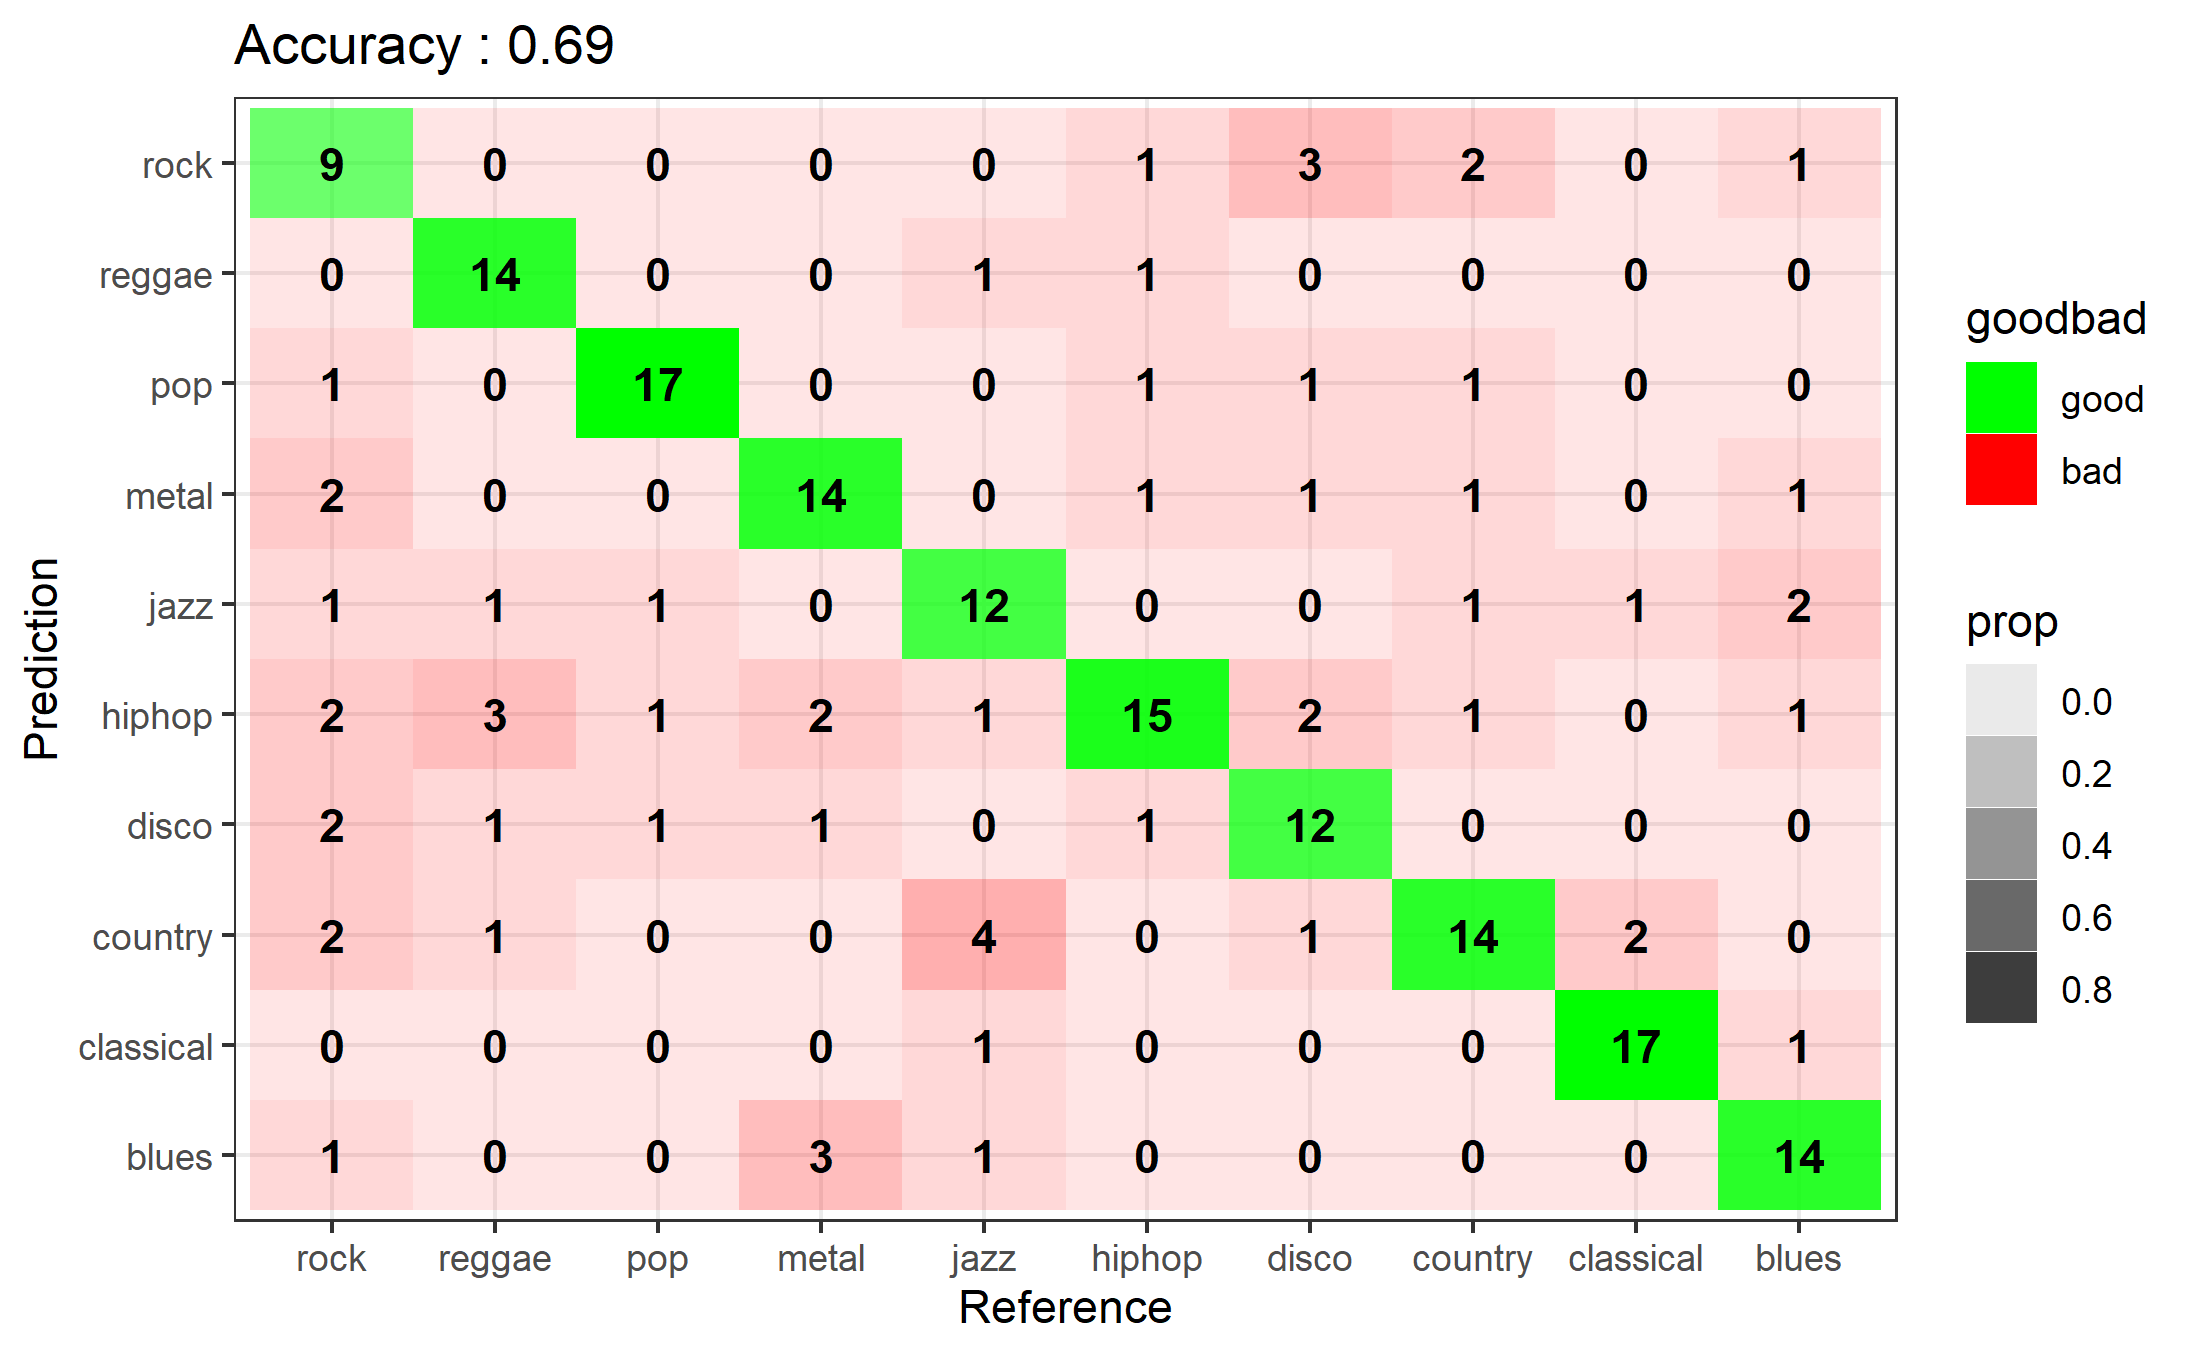
\includegraphics[width=0.9\textwidth]{confusionMatrix_randomforest.png}
\subsection{Random Forest(scaling)}
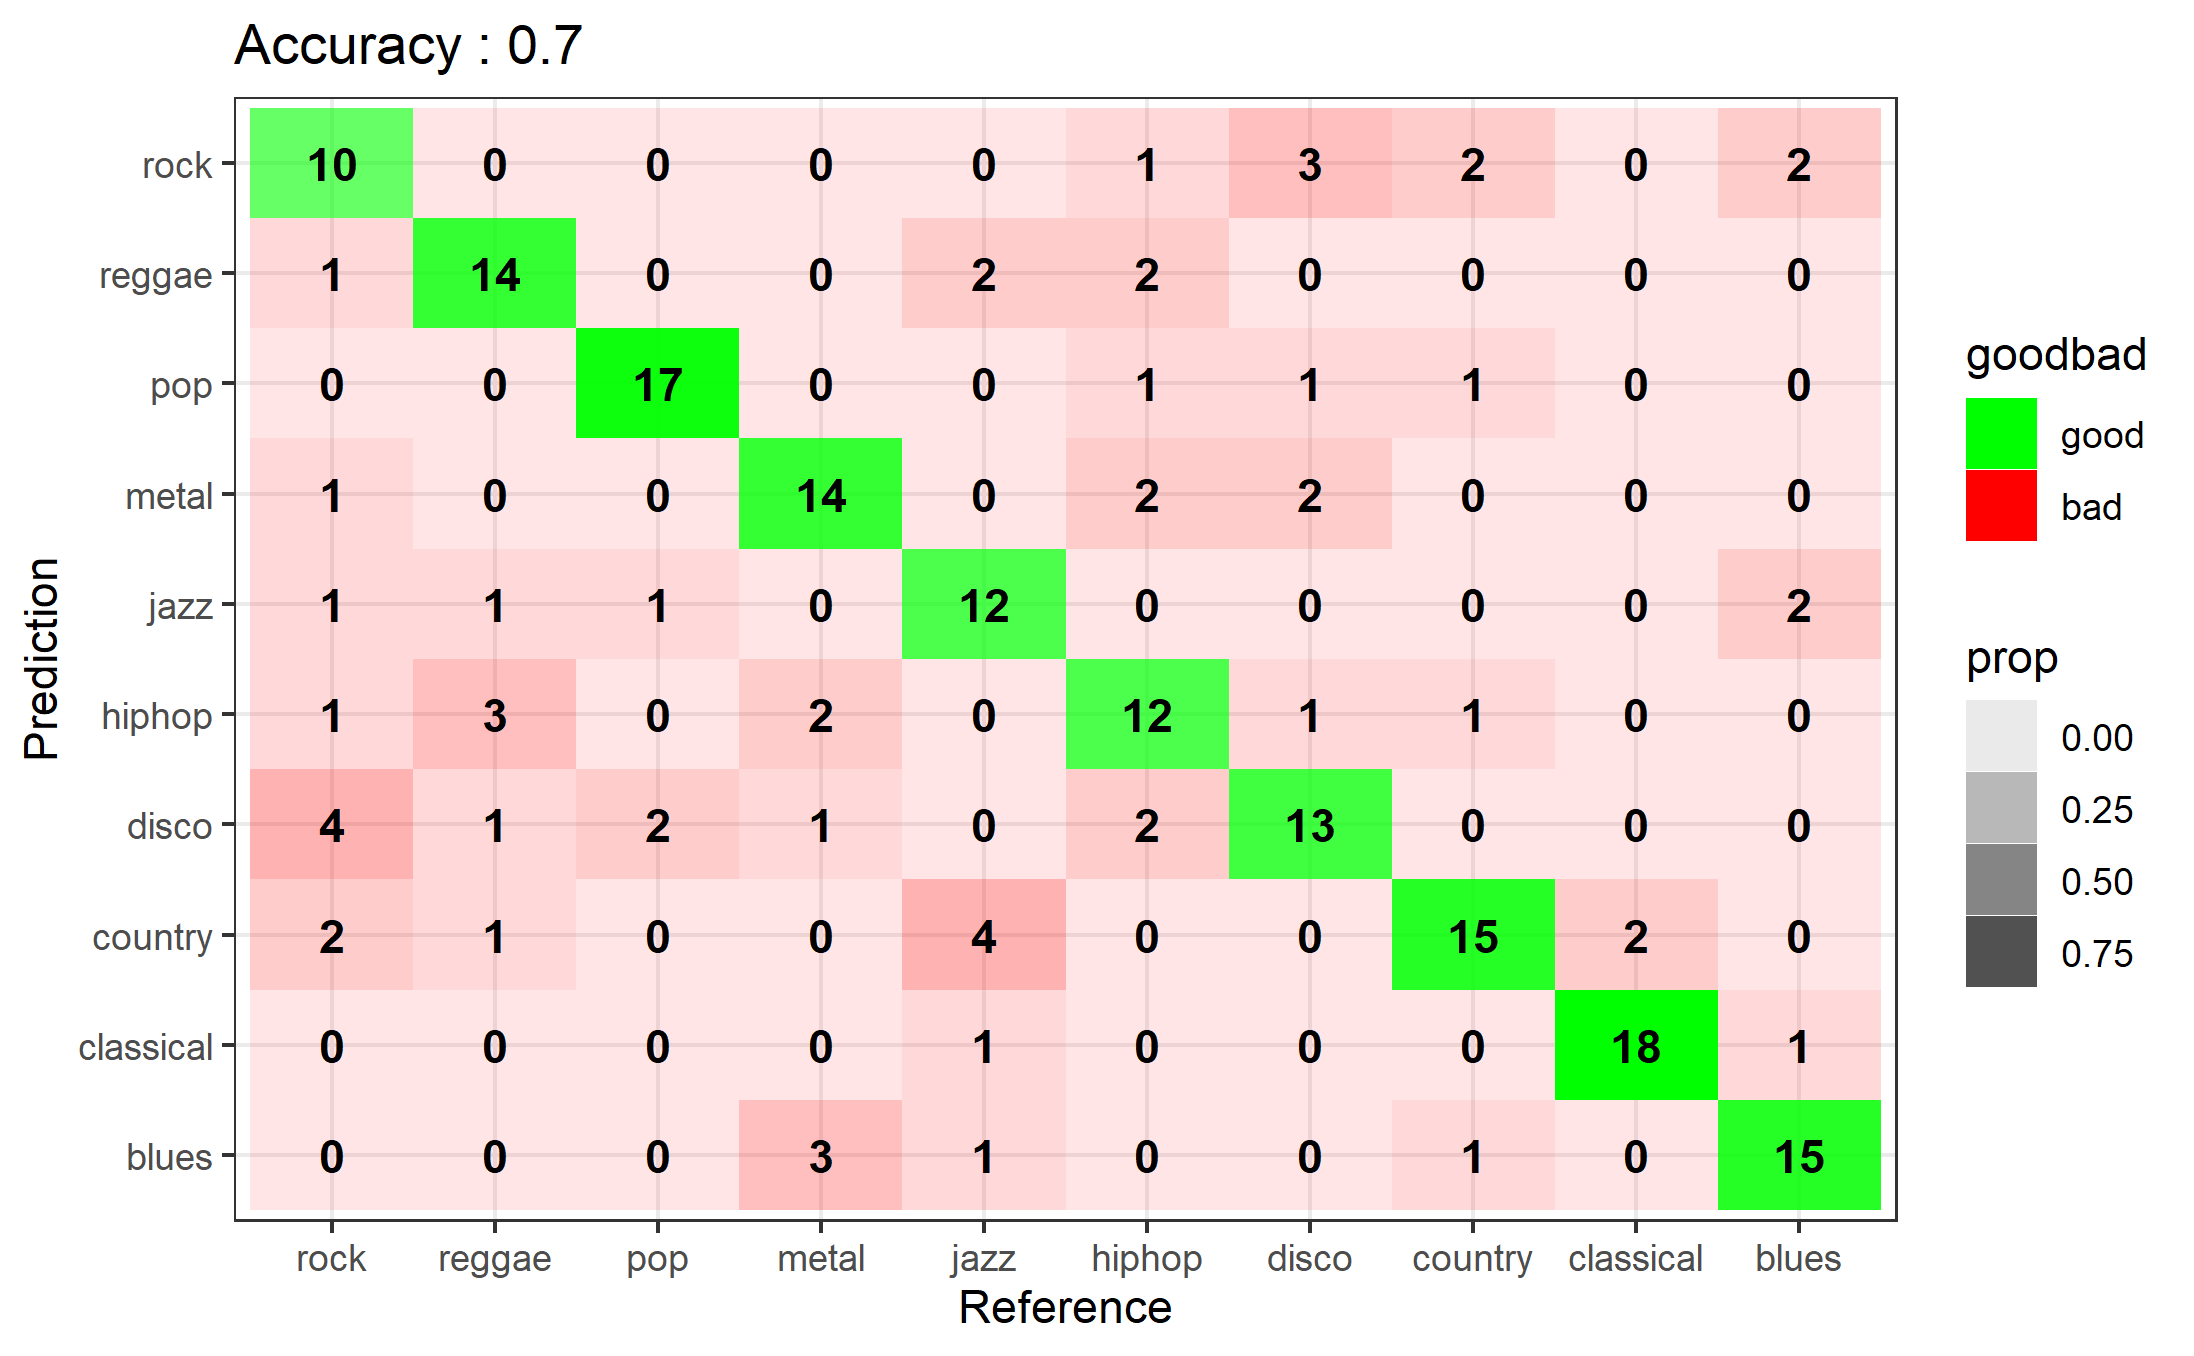
\includegraphics[width=0.9\textwidth]{confusionMatrix_randomforest_std.png}

\newpage
\section{Conclusion}
\begin{itemize}
  \item The music could be classified by those signal transform.
  \item SVM and Random Forest are nice classifier for this dataset.
\end{itemize}
\subsection{Results}
\begin{center}
\begin{tabular}{ |c|c| } 
\hline
 logistic regression & 0.55 \\ 
 \hline\hline
 svm(one-hot encoding) & 0.64 \\ 
 \hline
 svm & 0.67 \\ 
 \hline
 svm(scaling) & 0.69 \\ 
 \hline\hline
 random forest & 0.69 \\ 
 \hline
 random forest(scaling) & 0.7 \\ 
 \hline
\end{tabular}
\end{center}

\newpage
\section*{Reference}
\begin{itemize}
  \item (TextBook)Hastie, Tibshirani and Friedman (2009). The Elements of Statistical Learning: Data Mining, Inference and Prediction. 2nd Edition.
  \item (TextBook)Hardle and Simar (2015). Applied Multivariate Statistical Analysis, 4th Edition.
  \item (Paper)Chih-Wei Hsu, Chih-Chung Chang, and Chih-Jen Lin (2016). A Practical Guide to Support Vector Classification.
  \item  Meinard Muller, Stefan Balke (2015). Short-Time Fourier Transform and Chroma Features.
  \item (Website)Librosa
  \item (Website)Tempo vs Rhythm
\end{itemize}

\end{document}